\documentclass[12pt]{article}
\usepackage{amsmath}
\usepackage{graphicx}
\usepackage{hyperref}
\usepackage{listings}
\usepackage{color}
\usepackage{enumitem}
\usepackage{pythonhighlight}
\usepackage{xcolor}

\title{Operating System Course Report - First Half of the Semester}
\author{B class}
\date{\today}

\begin{document}

\maketitle
\newpage

\tableofcontents
\newpage

\section{Introduction}
This report summarizes the topics covered during the first half of the Operating System course. It includes theoretical concepts, practical implementations, and assignments. The course focuses on the fundamentals of operating systems, including system architecture, process management, CPU scheduling, and deadlock handling.

\section{Course Overview}
\subsection{Objectives}
The main objectives of this course are:
\begin{itemize}
    \item To understand the basic components and architecture of a computer system.
    \item To learn process management, scheduling, and inter-process communication.
    \item To explore file systems, input/output management, and virtualization.
    \item To study the prevention and handling of deadlocks in operating systems.
\end{itemize}

\subsection{Course Structure}
The course is divided into two halves. This report focuses on the first half, which covers:
\begin{itemize}
    \item Basic Concepts and Components of Computer Systems
    \item System Performance and Metrics
    \item System Architecture of Computer Systems
    \item Process Description and Control
    \item Scheduling Algorithms
    \item Process Creation and Termination
    \item Introduction to Threads
    \item File Systems
    \item Input and Output Management
    \item Deadlock Introduction and Prevention
    \item User Interface Management
    \item Virtualization in Operating Systems
\end{itemize}

\section{Topics Covered}

\subsection{Basic Concepts and Components of Computer Systems}
This section explains the fundamental components that make up a computer system, including the CPU, memory, storage, and input/output devices.

\subsection{System Performance and Metrics}
This section introduces various system performance metrics used to measure the efficiency of a computer system, including throughput, response time, and utilization.

\subsection{System Architecture of Computer Systems}
Describes the architecture of modern computer systems, focusing on the interaction between hardware and the operating system.

\subsection{Process Description and Control}
Processes are a central concept in operating systems. This section covers:
\begin{itemize}
    \item Process states and state transitions
    \item Process control block (PCB)
    \item Context switching
\end{itemize}

\subsection{Scheduling Algorithms}
This section covers:
\begin{itemize}
    \item First-Come, First-Served (FCFS)
    \item Shortest Job Next (SJN)
    \item Round Robin (RR)
\end{itemize}
It explains how these algorithms are used to allocate CPU time to processes.

\subsection{Process Creation and Termination}
Details how processes are created and terminated by the operating system, including:
\begin{itemize}
    \item Process spawning
    \item Process termination conditions
\end{itemize}

\subsection{Introduction to Threads}
This section introduces the concept of threads and their relation to processes, covering:
\begin{itemize}
    \item Single-threaded vs. multi-threaded processes
    \item Benefits of multithreading
\end{itemize}

\subsection{File Systems}
File systems provide a way for the operating system to store, retrieve, and manage data. This section explains:
\begin{itemize}
    \item File system structure
    \item File access methods
    \subsubsection*{3.8.3 Directory management}
    
    \begin{enumerate}
    \item \textbf{Direktori} \\
    Kumpulan file adalah direktori file. Direktori itu sendiri adalah file, dapat diakses oleh berbagai rutinitas manajemen file. Direktori berisi informasi tentang file, termasuk atribut, lokasi, dan kepemilikan. Sebagian besar informasi ini, terutama yang berkaitan dengan penyimpanan, dikelola oleh sistem operasi. Operasi direktori dapat mencari file, membuat file, menghapus file, mencantumkan direktori, mengganti nama file, dan melintasi sistem file.

    \item \textbf{Struktur Direktori}
    \begin{enumerate}[label=\alph*.]
        \item \textbf{Single-level Directory:} \\
        Karakteristik:
        \begin{itemize}
            \item Semua file dari semua pengguna disimpan dalam satu direktori yang sama.
            \item Dua file dengan nama yang sama tidak bisa disimpan di direktori yang sama.
            \item Struktur yang kurang fleksibel untuk pengorganisasi file yang lebih kompleks dan banyak pengguna.
        \end{itemize}
        
    \begin{figure}[h]
    \centering
    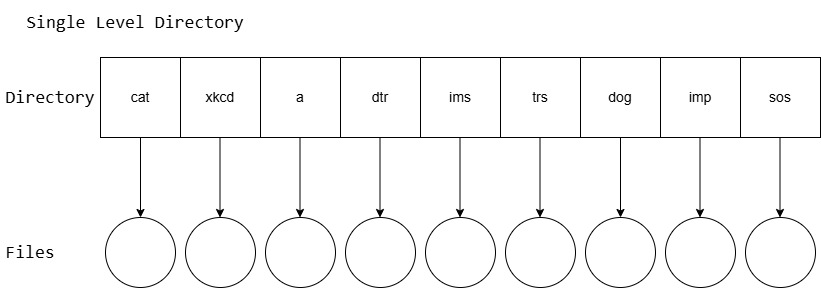
\includegraphics[width=0.5\textwidth]{asset/gambar1.jpg}
    \caption{Single Level Direktori.}
    \label{fig:single-level-direktori}
    \end{figure}

        \textbf{Penjelasan Gambar 1:}
        \begin{itemize}
            \item \textbf{Directory (Direktori):} Direktori diwakili oleh kotak besar di bagian atas, yang berisi beberapa nama file. Nama-nama seperti cat, xkcd, a, dtr, ims, trs, dog, imp, dan sos merupakan nama-nama file yang tersimpan dalam direktori tersebut.
            \item \textbf{Files (File):} File diwakili oleh lingkaran di bagian bawah, yang masing-masing terkait langsung dengan satu nama file di dalam direktori. Setiap file dalam direktori memiliki entri sendiri, namun semuanya berada di level yang sama dalam satu direktori.
        \end{itemize}

         \item \textbf{Two-level Directory:} \\
        Sistem ini memungkinkan setiap pengguna memiliki ruang penyimpanan terpisah untuk file mereka sendiri tanpa berbagi dengan pengguna lain.

        \begin{figure}[h]
        \centering
        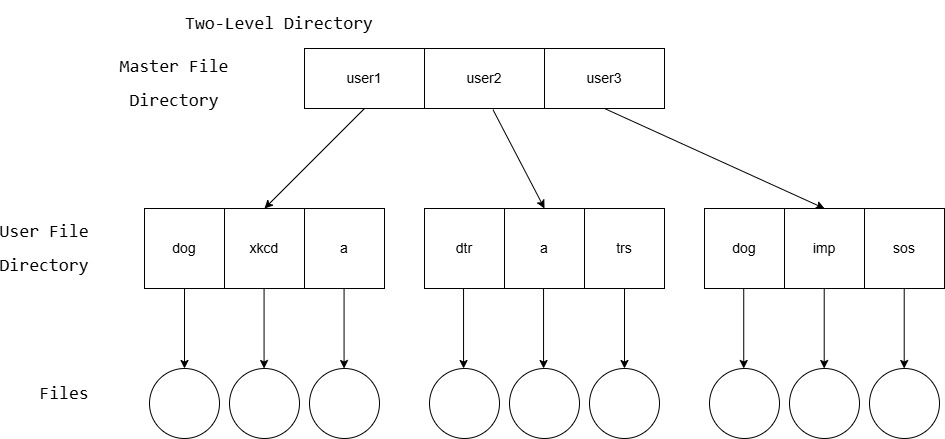
\includegraphics[width=0.5\textwidth]{asset/gambar2.jpg}
        \caption{Two-Level Direktori.}
        \label{fig:two-level-direktori}
        \end{figure}

        \textbf{Penjelasan Gambar 2:}
        \begin{itemize}
            \item \textbf{Master File Directory:} Bagian paling atas adalah direktori utama (master file directory) yang berisi daftar semua pengguna (user1, user2, user3). Ini seperti folder utama yang mencakup semua pengguna.
            \item \textbf{User File Directory:} Setiap pengguna (user1, user2, user3) memiliki direktori file mereka sendiri di dalam direktori utama. Ini disebut "User File Directory". Misalnya, user1 memiliki folder yang berisi "dog", "xkcd", dan "a".
            \item \textbf{Files:} Di dalam setiap "User File Directory", terdapat file-file yang dimiliki oleh pengguna tersebut. Misalnya, di dalam folder "dog" milik user1, terdapat file-file yang tidak ditampilkan detailnya dalam gambar (ditandai dengan lingkaran kosong).
        \end{itemize}

        \item \textbf{Tree-Structured Directory:} \\
        Karakteristik:
        \begin{itemize}
            \item \textbf{Hierarki yang Teratur:} Semua file dan direktori diatur secara hierarkis. Ini membantu dalam pengaturan file dan direktori dengan lebih baik.
            \item \textbf{Kemudahan Pengaturan Akses:} Pengaturan akses dan izin file dapat dikelola dengan lebih mudah karena setiap direktori memiliki hubungan hierarki yang jelas.
            \item \textbf{Pengelolaan Lebih Baik untuk Banyak Pengguna:} Setiap pengguna atau aplikasi bisa memiliki sub-direktori sendiri, memungkinkan isolasi dan keamanan file.
        \end{itemize}

        \begin{figure}[h]
        \centering
        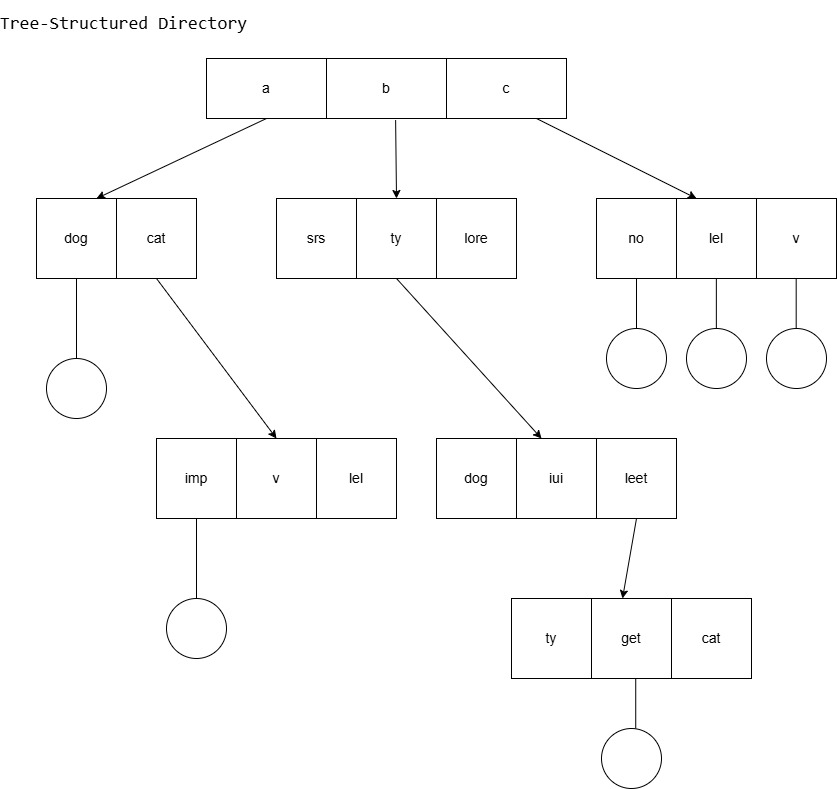
\includegraphics[width=0.5\textwidth]{asset/gambar3.jpg}
        \caption{Tree-Structured Direktori.}
        \label{fig:tree-structured-direktori}
        \end{figure}

        \textbf{Penjelasan Gambar 3:}
        \begin{itemize}
            \item \textbf{Root Directory:} Bagian paling atas dari struktur ini adalah direktori utama atau root, yang dalam gambar ini ditunjukkan oleh "a," "b," dan "c." Root directory adalah awal dari struktur pohon.
            \item \textbf{Subdirectories:} Setiap root directory memiliki sub-direktori. Misalnya:
            \begin{itemize}
                \item "a" memiliki sub-direktori "dog" dan "cat".
                \item "b" memiliki sub-direktori "srs," "ty," dan "lore".
                \item "c" memiliki sub-direktori "no," "lel," dan "v".
            \end{itemize}
            Sub-direktori ini dapat memiliki sub-direktori lain atau file di dalamnya. Misalnya, "cat" di bawah "a" memiliki sub-direktori imp, v, dan lel.
            \item \textbf{Files:} Setiap sub-direktori atau sub-folder dapat memiliki file atau bahkan sub-direktori lain yang membentuk struktur hierarki. Misalnya:
            \begin{itemize}
                \item Di bawah "dog" pada direktori "a," ada file.
                \item Di bawah "leet" pada direktori "b," ada sub-direktori "ty," "get," dan "cat."
            \end{itemize}
        \end{itemize}

        \item \textbf{Directory Graph Acyclic:} \\
        Struktur ini memungkinkan sebuah file atau direktori memiliki lebih dari satu nama atau jalur, yang disebut aliasing. Ini berarti bahwa file atau direktori bisa diakses melalui beberapa lokasi di dalam sistem file.

        Karakteristik Utama:
        \begin{itemize}
            \item \textbf{Aliasing:} Satu file dapat memiliki dua nama berbeda.
            \item \textbf{Pointer Gantung:} Jika satu jalur dihapus, pointer yang mengarah ke jalur tersebut menjadi tidak valid (dangling pointer).
            \item \textbf{Solusi untuk Pointer Gantung:}
            \begin{itemize}
                \item \textbf{Backpointers:} Menyimpan catatan asal setiap pointer agar bisa dihapus semua saat satu jalur dihapus.
                \item \textbf{Organisasi Daisy Chain:} Backpointers terhubung dalam bentuk rantai.
                \item \textbf{Entry-hold-count:} Sistem menghitung jumlah link ke setiap file atau direktori, dan hanya menghapus file jika jumlahnya nol.
            \end{itemize}
            \item \textbf{Link Baru:} Entri direktori bisa berisi link, yaitu pointer ke file lain. Sistem harus resolve link untuk menemukan file yang sebenarnya.
        \end{itemize}

        Struktur ini memecahkan masalah penyimpanan data secara efisien dengan mendukung penggunaan beberapa jalur untuk file yang sama, namun perlu manajemen yang baik untuk mencegah pointer gantung.
    \end{enumerate}
\end{enumerate}
        
\end{itemize}

\subsection{Input and Output Management}
Input and output management is key for handling the interaction between the system and external devices. This section includes:
\begin{itemize}
    \item Device drivers
    \item I/O scheduling
\end{itemize}

\subsection{Deadlock Introduction and Prevention}
Explores the concept of deadlocks and methods for preventing them:
\begin{itemize}
    \item Deadlock conditions
    \item Deadlock prevention techniques
\end{itemize}

\subsection{User Interface Management}
This section discusses the role of the operating system in managing the user interface. Topics covered include:
\begin{itemize}
    \item Graphical User Interface (GUI)
    \item Command-Line Interface (CLI)
    \item Interaction between the user and the operating system
\end{itemize}

\subsection{Virtualization in Operating Systems}
Virtualization allows multiple operating systems to run concurrently on a single physical machine. This section explores:
\begin{itemize}
    \item Concept of virtualization
    \item Hypervisors and their types
    \item Benefits of virtualization in modern computing
\end{itemize}

\section{Assignments and Practical Work}
\subsection{Assignment 1: Process Scheduling}
Students were tasked with implementing various process scheduling algorithms (e.g., FCFS, SJN, and RR) and comparing their performance under different conditions.
\subsubsection{Group 1}
\begin{python}
    class Process:
    def _init_(self, pid, arrival_time, burst_time):
        self.pid = pid
        self.arrival_time = arrival_time
        self.burst_time = burst_time
        self.completion_time = 0
        self.turnaround_time = 0
        self.waiting_time = 0
\end{python}

\begin{table}[htbp] % Optional: For floating position
    \centering
    \begin{tabular}{|c|c|c|} % Defines number of columns and alignment (c = center, l = left, r = right). '|' creates vertical lines.
    \hline
    Header 1 & Header 2 & Header 3 \\ % Column headers
    \hline
    Row 1, Column 1 & Row 1, Column 2 & Row 1, Column 3 \\ % First row of data
    \hline
    Row 2, Column 1 & Row 2, Column 2 & Row 2, Column 3 \\ % Second row of data
    \hline
    \end{tabular}
    \caption{Your table caption} % Optional: For adding a caption
    \label{tab:your_label} % Optional: For cross-referencing the table
\end{table}

\subsection{Assignment 2: Deadlock Handling}
In this assignment, students were asked to simulate different deadlock scenarios and explore various prevention methods.

\subsubsection{Group 8}
\begin{enumerate}[label=\alph*.]
\item  \textbf{Soal} \\
Di sebuah bank, terdapat empat proses yang menangani berbagai layanan seperti transaksi penarikan, setoran, dan transfer. Masing-masing proses membutuhkan sumber daya seperti jaringan, basis data, dan API eksternal untuk menyelesaikan transaksi mereka.

Kejadian deadlock mungkin terjadi jika proses saling menunggu sumber daya yang sudah dimiliki oleh proses lain. Tugasnya adalah membuat program Python untuk mendeteksi apakah terjadi deadlock dalam skenario ini menggunakan Wait-for Graph.

\begin{itemize}
    \item Proses 1 (P1) membutuhkan akses ke jaringan dan basis data.
    \item Proses 2 (P2) membutuhkan akses ke API eksternal dan basis data.
    \item Proses 3 (P3) membutuhkan akses ke basis data dan jaringan.
    \item Proses 4 (P4) membutuhkan akses ke jaringan dan API eksternal.
\end{itemize}


    \item \textbf{Jawaban (Python)}
\begin{lstlisting}[language=Python, caption=Deadlock Detection in Python, label=lst:pythoncode, frame=single, backgroundcolor=\color{lightgray}, basicstyle=\ttfamily\small, breaklines=true, xleftmargin=1em, xrightmargin=1em]
# Fungsi untuk mendeteksi siklus (deadlock) menggunakan algoritma DFS
def detect_cycle(wait_for_graph, visited, rec_stack, process):
    visited[process] = True
    rec_stack[process] = True

    # Mengecek semua proses yang sedang menunggu proses ini
    for neighbor in wait_for_graph[process]:
        if not visited[neighbor]:
            if detect_cycle(wait_for_graph, visited, rec_stack, neighbor):
                return True
        elif rec_stack[neighbor]:
            return True

    rec_stack[process] = False
    return False

# Fungsi utama untuk mendeteksi deadlock
def deadlock_detection(processes, wait_for_graph):
    visited = {p: False for p in processes}
    rec_stack = {p: False for p in processes}

    # Melakukan DFS dari setiap proses
    for process in processes:
        if not visited[process]:
            if detect_cycle(wait_for_graph, visited, rec_stack, process):
                return True
    return False

# Input: Proses dan Wait-for Graph
processes = ['P1', 'P2', 'P3', 'P4']
wait_for_graph = {
    'P1': ['P3'],  # P1 menunggu P3
    'P2': ['P1'],  # P2 menunggu P1
    'P3': ['P4'],  # P3 menunggu P4
    'P4': ['P2'],  # P4 menunggu P2 (membentuk siklus)
}

# Memeriksa apakah ada deadlock
if deadlock_detection(processes, wait_for_graph):
    print("Deadlock terdeteksi! Proses-proses yang terlibat: P1, P2, P3, P4")
else:
    print("Tidak ada deadlock.")
\end{lstlisting}

\item \textbf{Output} \\
Berikut adalah output dari program deteksi deadlock yang dijalankan:
\begin{verbatim}
Deadlock terdeteksi! Proses-proses yang terlibat: P1, P2, P3, P4
\end{verbatim}
\end{enumerate}

\subsection{Assignment 3: Multithreading and Amdahl's Law}
This assignment involved designing a multithreading scenario to solve a computationally intensive problem. Students then applied **Amdahl's Law** to calculate the theoretical speedup of the program as the number of threads increased.

\subsection{Assignment 4: Simple Command-Line Interface (CLI) for User Interface Management}
Students were tasked with creating a simple **CLI** for user interface management. The CLI should support basic commands such as file manipulation (creating, listing, and deleting files), process management, and system status reporting.

\subsection{Assignment 5: File System Access}
In this assignment, students implemented file system access routines, including:
\begin{itemize}
    \item File creation and deletion
    \item Reading from and writing to files
    \item Navigating directories and managing file permissions
\end{itemize}

\section{Conclusion}
The first half of the course introduced core operating system concepts, including process management, scheduling, multithreading, and file system access. These topics provided a foundation for more advanced topics to be covered in the second half of the course.

\section{Referensi}
\sloppy
\begin{itemize}
    \item {Silberschatz, dkk. 2013. Chapter 10 : File System. Operating System Concepts - 9th Edition.}
    \item {Yadav, Aakansha. 2024. File Systems in Operating System. https://www.geeksforgeeks.org/file-systems-in-operating-system/. Diakses : 08 September 2024.}
\end{itemize}
\fussy

\end{document}